\documentclass[12pt]{article}
\usepackage[a4paper,margin=2.5cm]{geometry}
\usepackage{amsmath, amssymb, amsthm}
\usepackage{bm}
\usepackage{hyperref}
\usepackage{graphicx}
\usepackage{caption}
\usepackage{listings}
\usepackage{xcolor}
\usepackage{float}
\usepackage{placeins}
\graphicspath{{figures/}}

% Code style
\lstdefinestyle{code}{
  basicstyle=\ttfamily\small,
  numbers=left,
  numberstyle=\tiny,
  numbersep=8pt,
  keywordstyle=\color{blue},
  commentstyle=\color{teal!70!black},
  stringstyle=\color{orange!70!black},
  showstringspaces=false,
  breaklines=true,
  frame=single,
  framerule=0.3pt,
  rulecolor=\color{black!15}
}
\lstset{style=code}

\title{Training Deep Networks Tutorial}
\author{}
\date{\today}

\begin{document}
\maketitle

\section{Backpropagation Algorithm}
Backpropagation applies the chain rule to efficiently compute gradients of a scalar loss $\mathcal{L}$ with respect to all network parameters. Consider an $L$-layer MLP with activations $\mathbf{h}^{(\ell)} = \phi^{(\ell)}(\mathbf{a}^{(\ell)})$ and pre-activations $\mathbf{a}^{(\ell)} = \mathbf{W}^{(\ell)} \mathbf{h}^{(\ell-1)} + \mathbf{b}^{(\ell)}$. The loss gradient with respect to pre-activations is propagated backward as
\begin{equation}
  \boldsymbol{\delta}^{(\ell)} = \bigl(\mathbf{W}^{(\ell+1)}\bigr)^{\top} \boldsymbol{\delta}^{(\ell+1)} \odot \phi'^{(\ell)}\bigl(\mathbf{a}^{(\ell)}\bigr),
\end{equation}
where $\odot$ denotes element-wise multiplication and $\boldsymbol{\delta}^{(L)} = \nabla_{\mathbf{h}^{(L)}} \mathcal{L}$. Parameter gradients follow directly:
\begin{align}
  \nabla_{\mathbf{W}^{(\ell)}} \mathcal{L} &= \boldsymbol{\delta}^{(\ell)} \bigl(\mathbf{h}^{(\ell-1)}\bigr)^{\top}, \\
  \nabla_{\mathbf{b}^{(\ell)}} \mathcal{L} &= \boldsymbol{\delta}^{(\ell)}.
\end{align}
The computational graph in Figure~\ref{fig:backprop_graph} highlights the forward and backward flows.

The vector-Jacobian product perspective generalizes to arbitrary architectures: given intermediate variable $\mathbf{z}$ with local Jacobian $\mathbf{J} = \partial \mathbf{z} / \partial \boldsymbol{\theta}$, backprop multiplies the upstream gradient by $\mathbf{J}$ without explicitly forming it, yielding $\nabla_{\boldsymbol{\theta}} \mathcal{L} = \mathbf{J}^{\top} \nabla_{\mathbf{z}} \mathcal{L}$.

\begin{lstlisting}[language=Python, caption={Mini-batch backprop for a dense network.}]
def backward_pass(weights, activations, preacts, grads_out, loss_grad):
    deltas = [None] * len(weights)
    deltas[-1] = loss_grad
    for l in reversed(range(len(weights) - 1)):
        W_next = weights[l + 1]
        delta_next = deltas[l + 1]
        deltas[l] = (W_next.T @ delta_next) * activations[l] * (1 - activations[l])
    grad_W = [delta @ a.T for delta, a in zip(deltas, preacts)]
    grad_b = [delta.sum(axis=1, keepdims=True) for delta in deltas]
    return grad_W, grad_b
\end{lstlisting}

\begin{figure}[H]
  \centering
  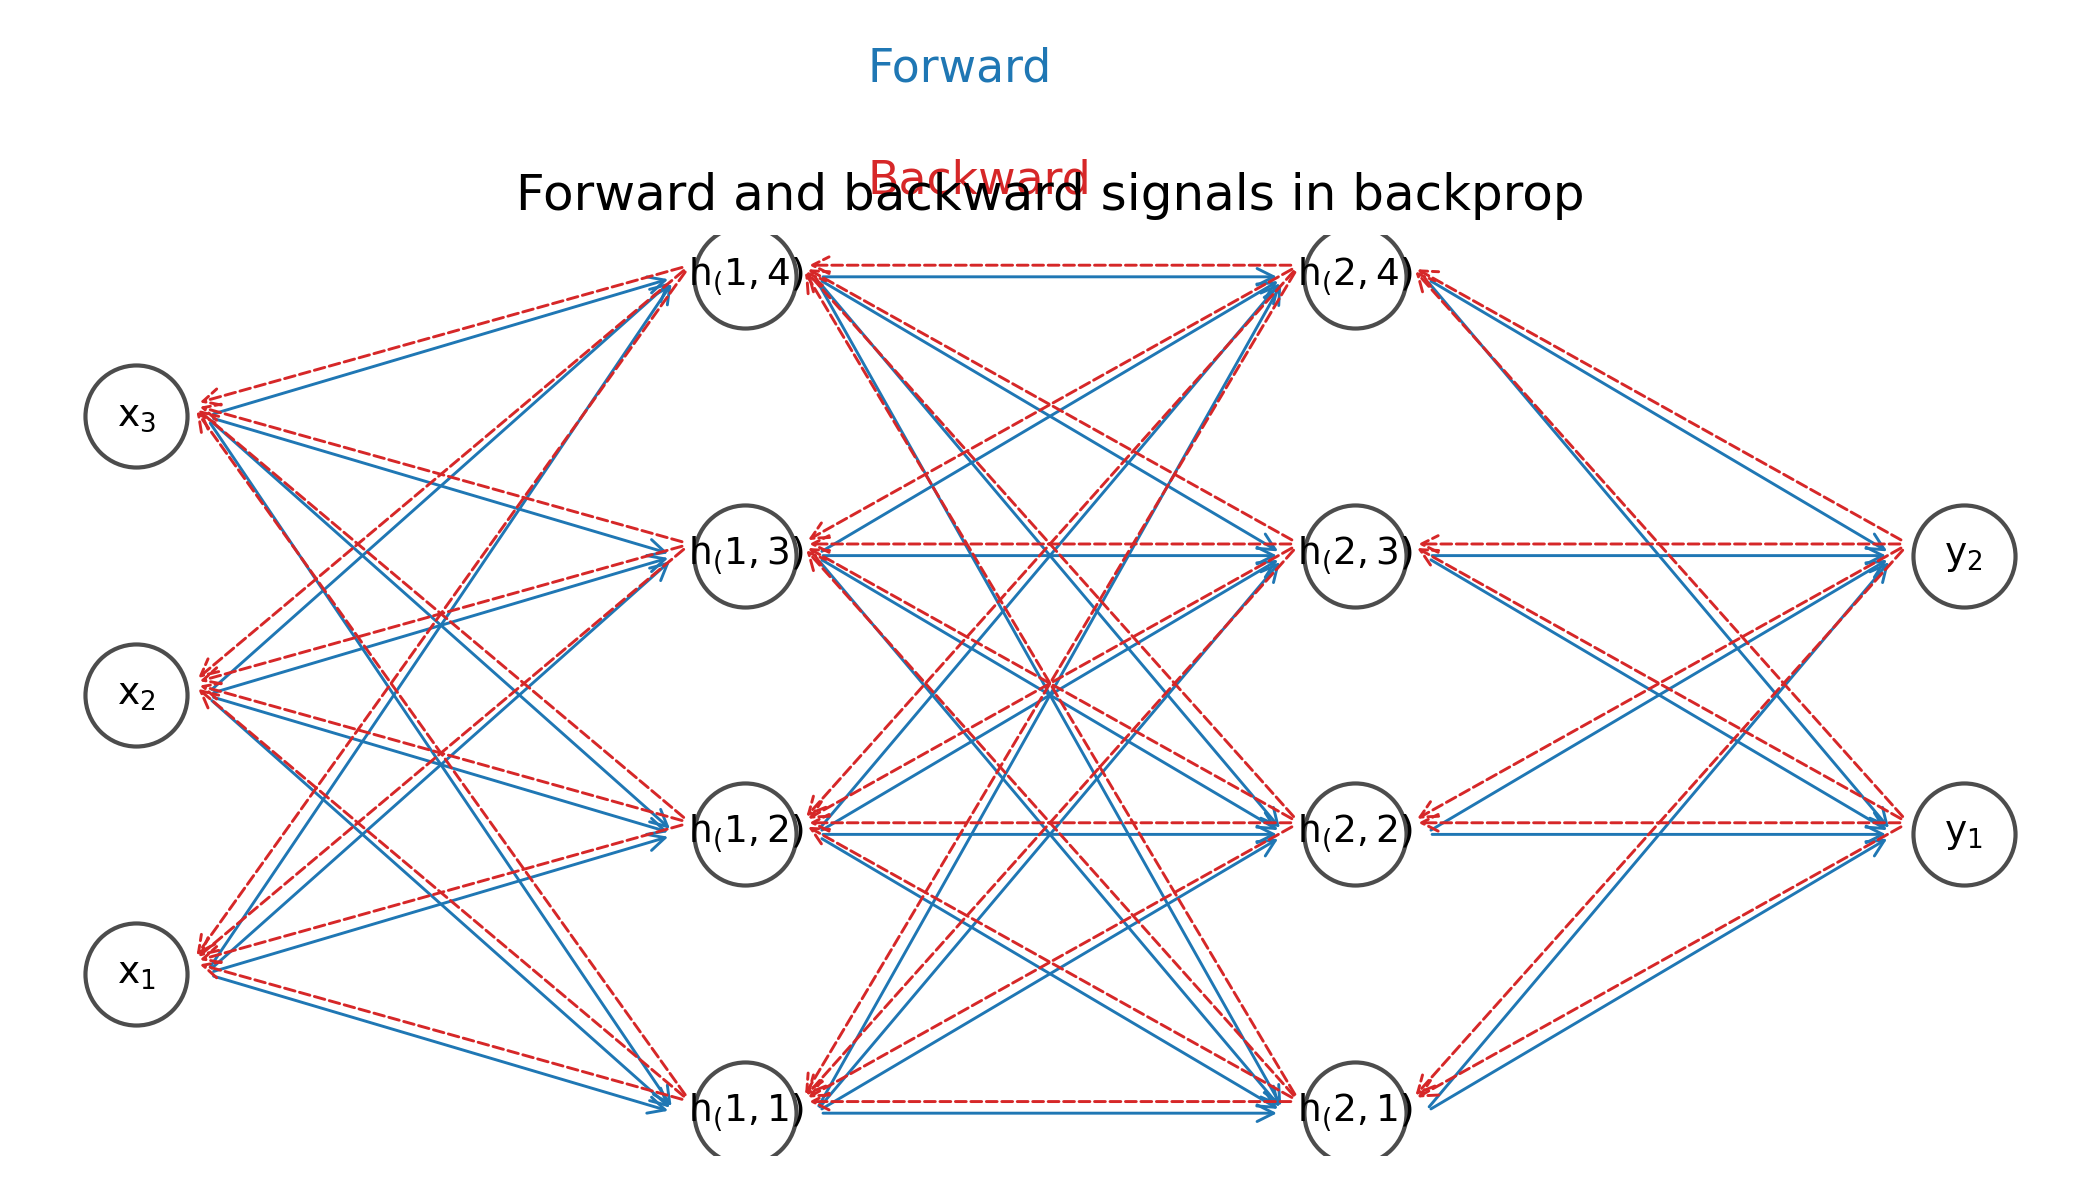
\includegraphics[width=0.8\linewidth]{backprop_computational_graph.png}
  \caption{Forward (solid) and backward (dashed) flows through a layered network.}
  \label{fig:backprop_graph}
\end{figure}
\FloatBarrier

\section{Gradient Descent Methods}
Given gradients $\nabla_{\boldsymbol{\theta}} \mathcal{L}$, parameters are updated iteratively to minimize the loss. Figure~\ref{fig:optimization_trajectories} compares optimization paths.

\subsection{Stochastic Gradient Descent (SGD)}
SGD uses noisy gradient estimates from mini-batches:
\begin{equation}
  \boldsymbol{\theta}_{t+1} = \boldsymbol{\theta}_t - \eta_t \nabla_{\boldsymbol{\theta}} \mathcal{L}(\boldsymbol{\theta}_t; \mathcal{B}_t).
\end{equation}
The learning rate $\eta_t$ may be constant or scheduled. Noise from sampling promotes exploration of flatter minima but can slow convergence.

\subsection{Momentum}
Momentum accumulates a velocity vector $\mathbf{v}_t$ to smooth gradients:
\begin{align}
  \mathbf{v}_{t+1} &= \mu \mathbf{v}_t - \eta_t \nabla_{\boldsymbol{\theta}} \mathcal{L}(\boldsymbol{\theta}_t), \\
  \boldsymbol{\theta}_{t+1} &= \boldsymbol{\theta}_t + \mathbf{v}_{t+1},
\end{align}
where $\mu \in [0,1)$ is the momentum coefficient. Momentum accelerates progress along persistent descent directions while damping oscillations in steep ravines.

\subsection{Nesterov Accelerated Gradient (NAG)}
Nesterov momentum anticipates the effect of the velocity:
\begin{align}
  \tilde{\boldsymbol{\theta}}_t &= \boldsymbol{\theta}_t + \mu \mathbf{v}_t, \\
  \mathbf{v}_{t+1} &= \mu \mathbf{v}_t - \eta_t \nabla_{\boldsymbol{\theta}} \mathcal{L}(\tilde{\boldsymbol{\theta}}_t), \\
  \boldsymbol{\theta}_{t+1} &= \boldsymbol{\theta}_t + \mathbf{v}_{t+1}.
\end{align}
Evaluating the gradient at the look-ahead position provides stronger theoretical guarantees and often yields faster convergence in practice.

\begin{figure}[H]
  \centering
  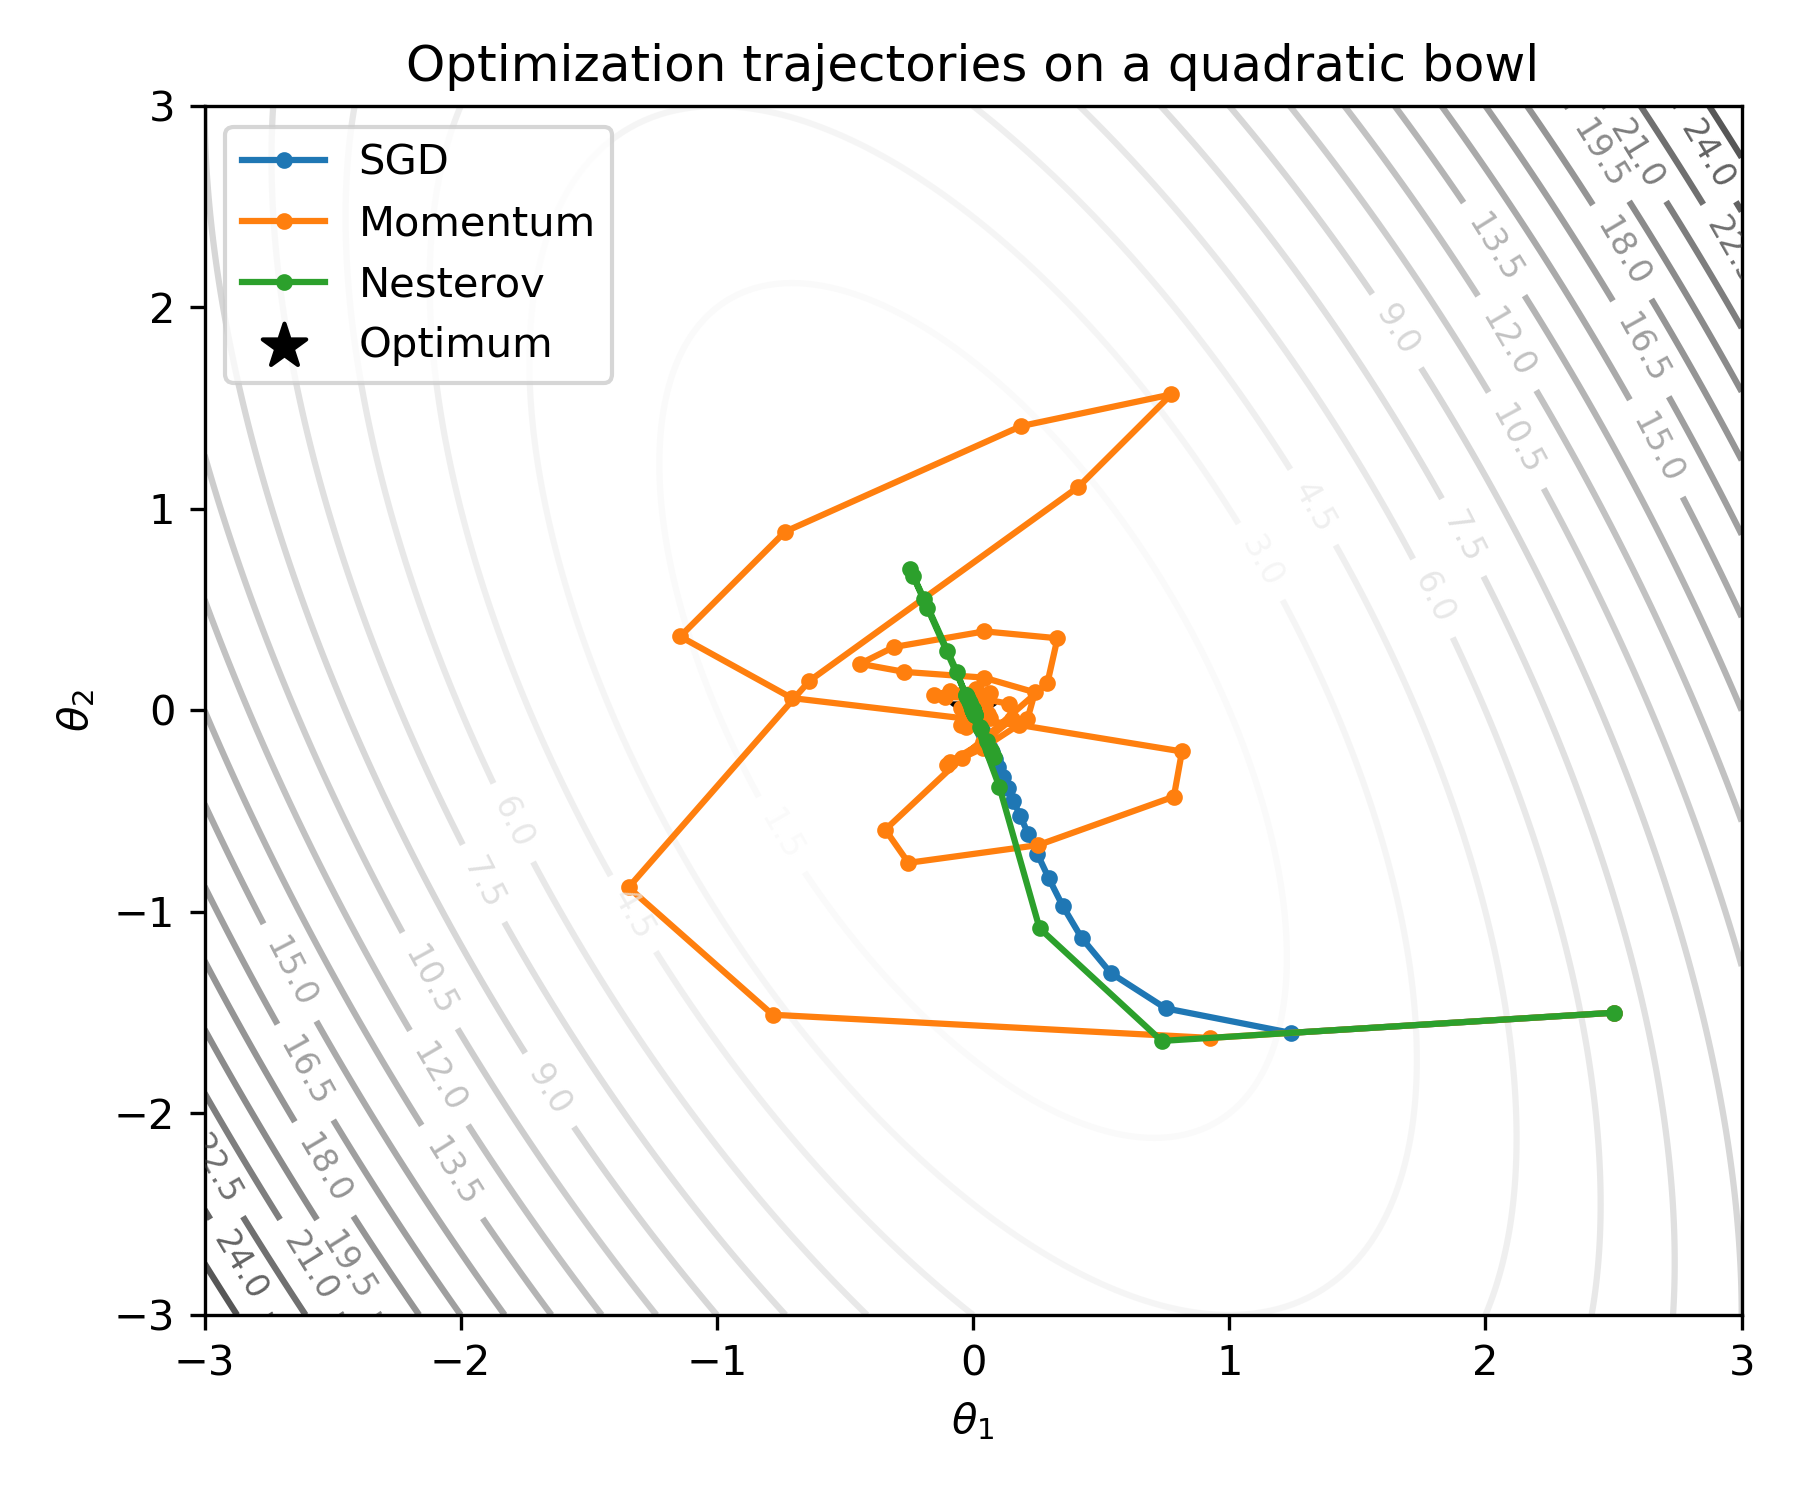
\includegraphics[width=0.8\linewidth]{optimization_trajectories.png}
  \caption{Optimization paths of SGD variants on a curved quadratic landscape.}
  \label{fig:optimization_trajectories}
\end{figure}
\FloatBarrier

\section{Learning Rate Scheduling}
Effective schedules balance rapid initial descent with stable convergence. Common strategies include:

\begin{itemize}
  \item \textbf{Step decay:} reduce $\eta$ by a factor $\gamma < 1$ every $k$ epochs, \(\eta_t = \eta_0 \gamma^{\lfloor t/k \rfloor}\).
  \item \textbf{Exponential decay:} continuously decrease $\eta_t = \eta_0 \exp(-\lambda t)$.
  \item \textbf{Cosine annealing:} use a cosine cycle between $\eta_{\min}$ and $\eta_{\max}$ with optional restarts.
  \item \textbf{Warmup:} linearly increase $\eta$ over the first $T_w$ steps before applying the main schedule.
\end{itemize}

Figure~\ref{fig:lr_schedules} visualizes several schedules and their warmup phases. Adaptive optimizers (Adam, RMSprop) implicitly adjust learning rates per parameter, yet explicit schedules remain beneficial.

\begin{figure}[H]
  \centering
  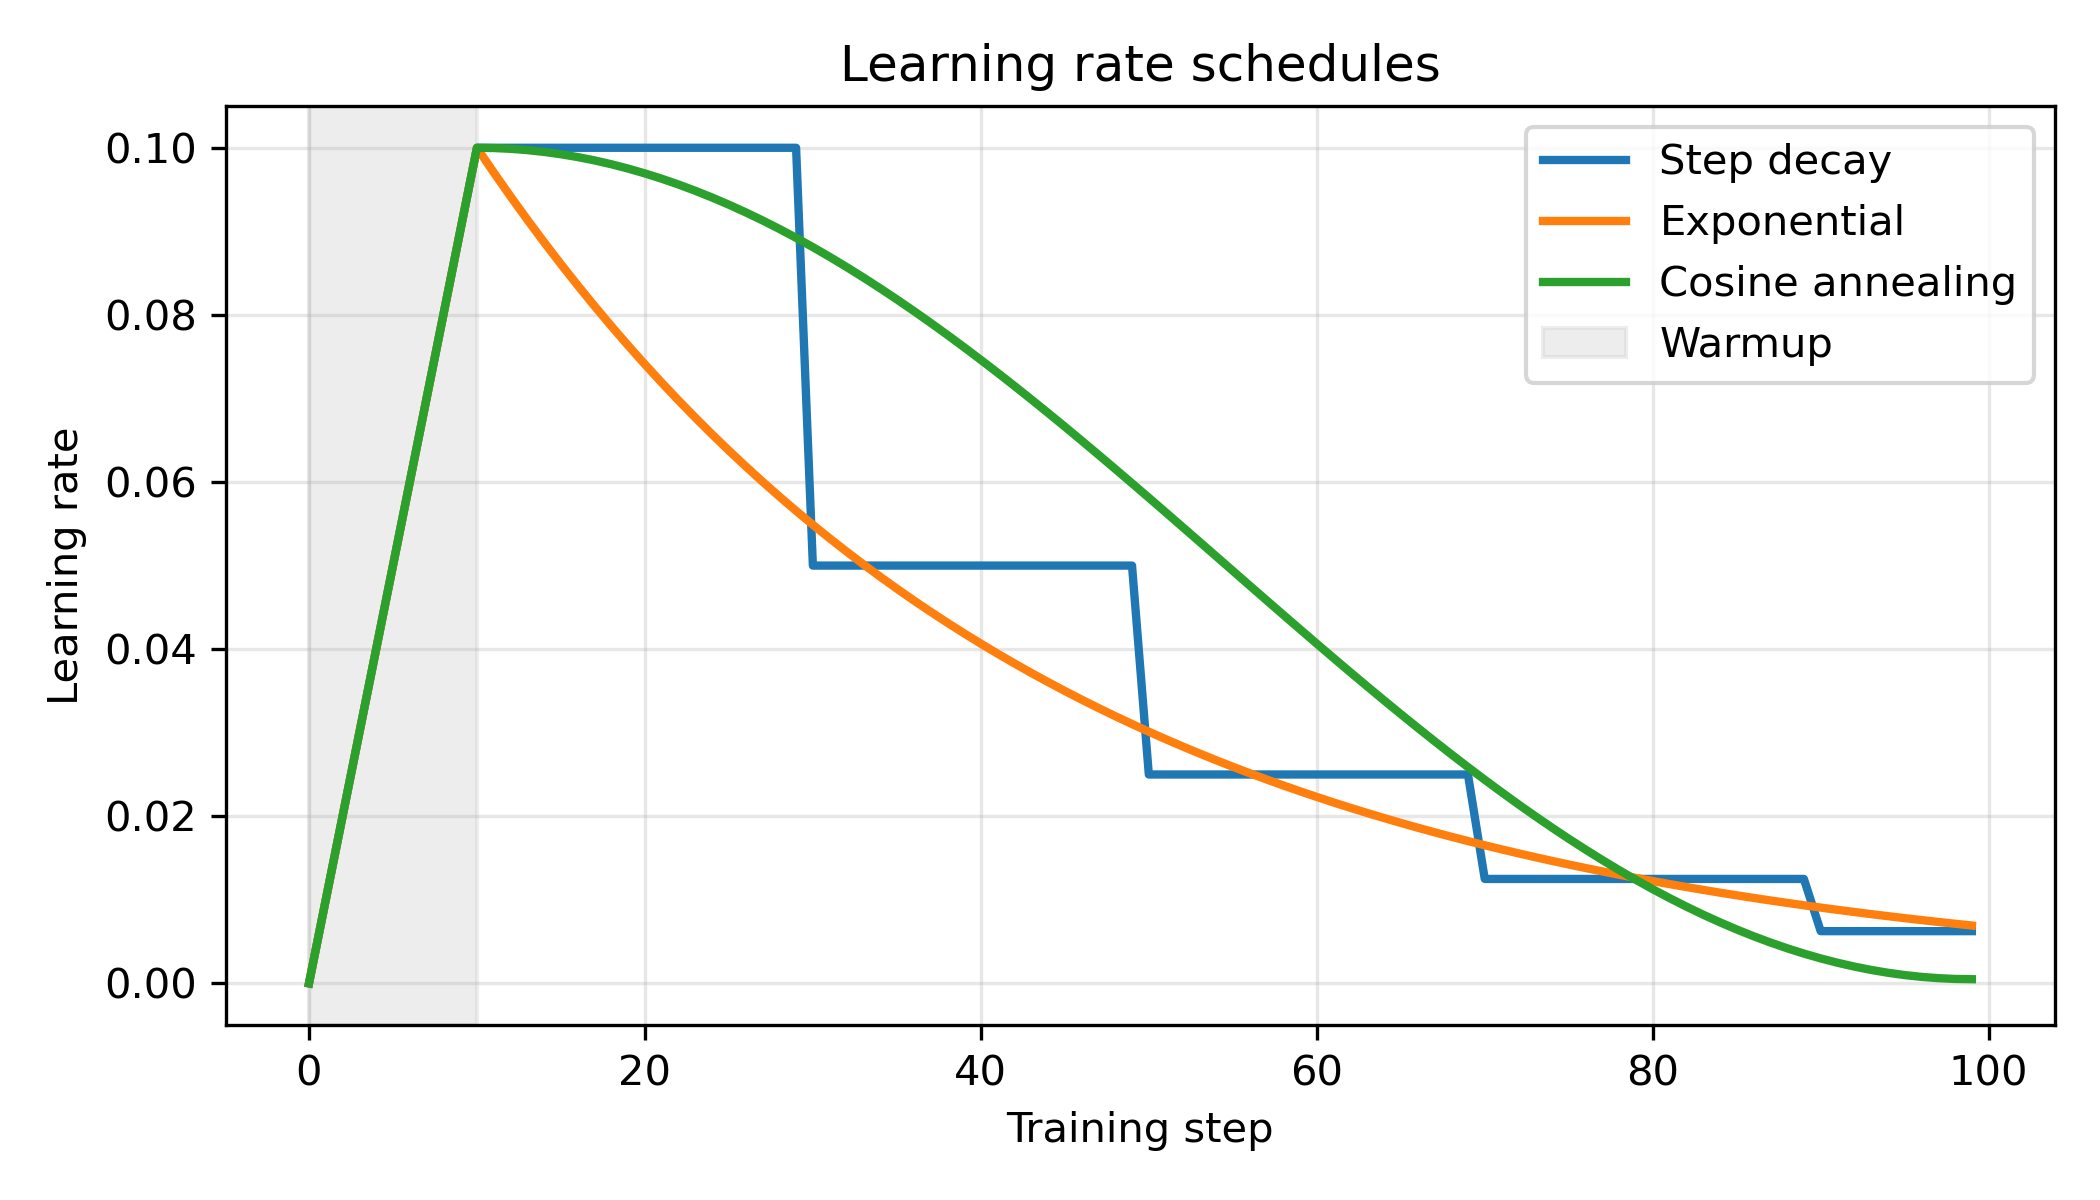
\includegraphics[width=0.8\linewidth]{learning_rate_schedules.png}
  \caption{Examples of learning rate schedules with linear warmup.}
  \label{fig:lr_schedules}
\end{figure}
\FloatBarrier

\section{Overfitting and Regularization}
Overfitting occurs when a model memorizes training data but fails to generalize. Figure~\ref{fig:regularization_effects} illustrates how regularizers reduce the generalization gap.

\subsection{Weight Penalties}
L2 regularization adds $\lambda \|\boldsymbol{\theta}\|_2^2$ to the loss, yielding parameter shrinkage equivalent to weight decay. L1 regularization adds $\lambda \|\boldsymbol{\theta}\|_1$, promoting sparsity. Both translate into modified gradients:
\begin{align}
  \nabla_{\boldsymbol{\theta}} (\mathcal{L} + \lambda \|\boldsymbol{\theta}\|_2^2) &= \nabla_{\boldsymbol{\theta}} \mathcal{L} + 2\lambda \boldsymbol{\theta}, \\
  \nabla_{\boldsymbol{\theta}} (\mathcal{L} + \lambda \|\boldsymbol{\theta}\|_1) &= \nabla_{\boldsymbol{\theta}} \mathcal{L} + \lambda\, \mathrm{sign}(\boldsymbol{\theta}).
\end{align}

\subsection{Dropout}
Dropout randomly zeros activations during training with keep probability $p$, sampling masks $\mathbf{m} \sim \mathrm{Bernoulli}(p)$ and computing $\tilde{\mathbf{h}} = \mathbf{m} \odot \mathbf{h}$. At inference time activations are scaled by $p$. Dropout discourages co-adaptation and approximates an ensemble of subnetworks.

\subsection{Data Augmentation}
Augmentations expand the training distribution through label-preserving transformations (crops, flips, color jitter). They inject inductive biases and reduce variance without altering the model.

\subsection{Batch Normalization}
BatchNorm normalizes activations using batch statistics:
\begin{align}
  \hat{\mathbf{h}} &= \frac{\mathbf{h} - \boldsymbol{\mu}_\mathcal{B}}{\sqrt{\boldsymbol{\sigma}_\mathcal{B}^2 + \epsilon}}, \\
  \mathbf{y} &= \boldsymbol{\gamma} \odot \hat{\mathbf{h}} + \boldsymbol{\beta}.
\end{align}
By stabilizing activation distributions, BatchNorm allows higher learning rates and provides regularization via batch noise.

\begin{figure}[H]
  \centering
  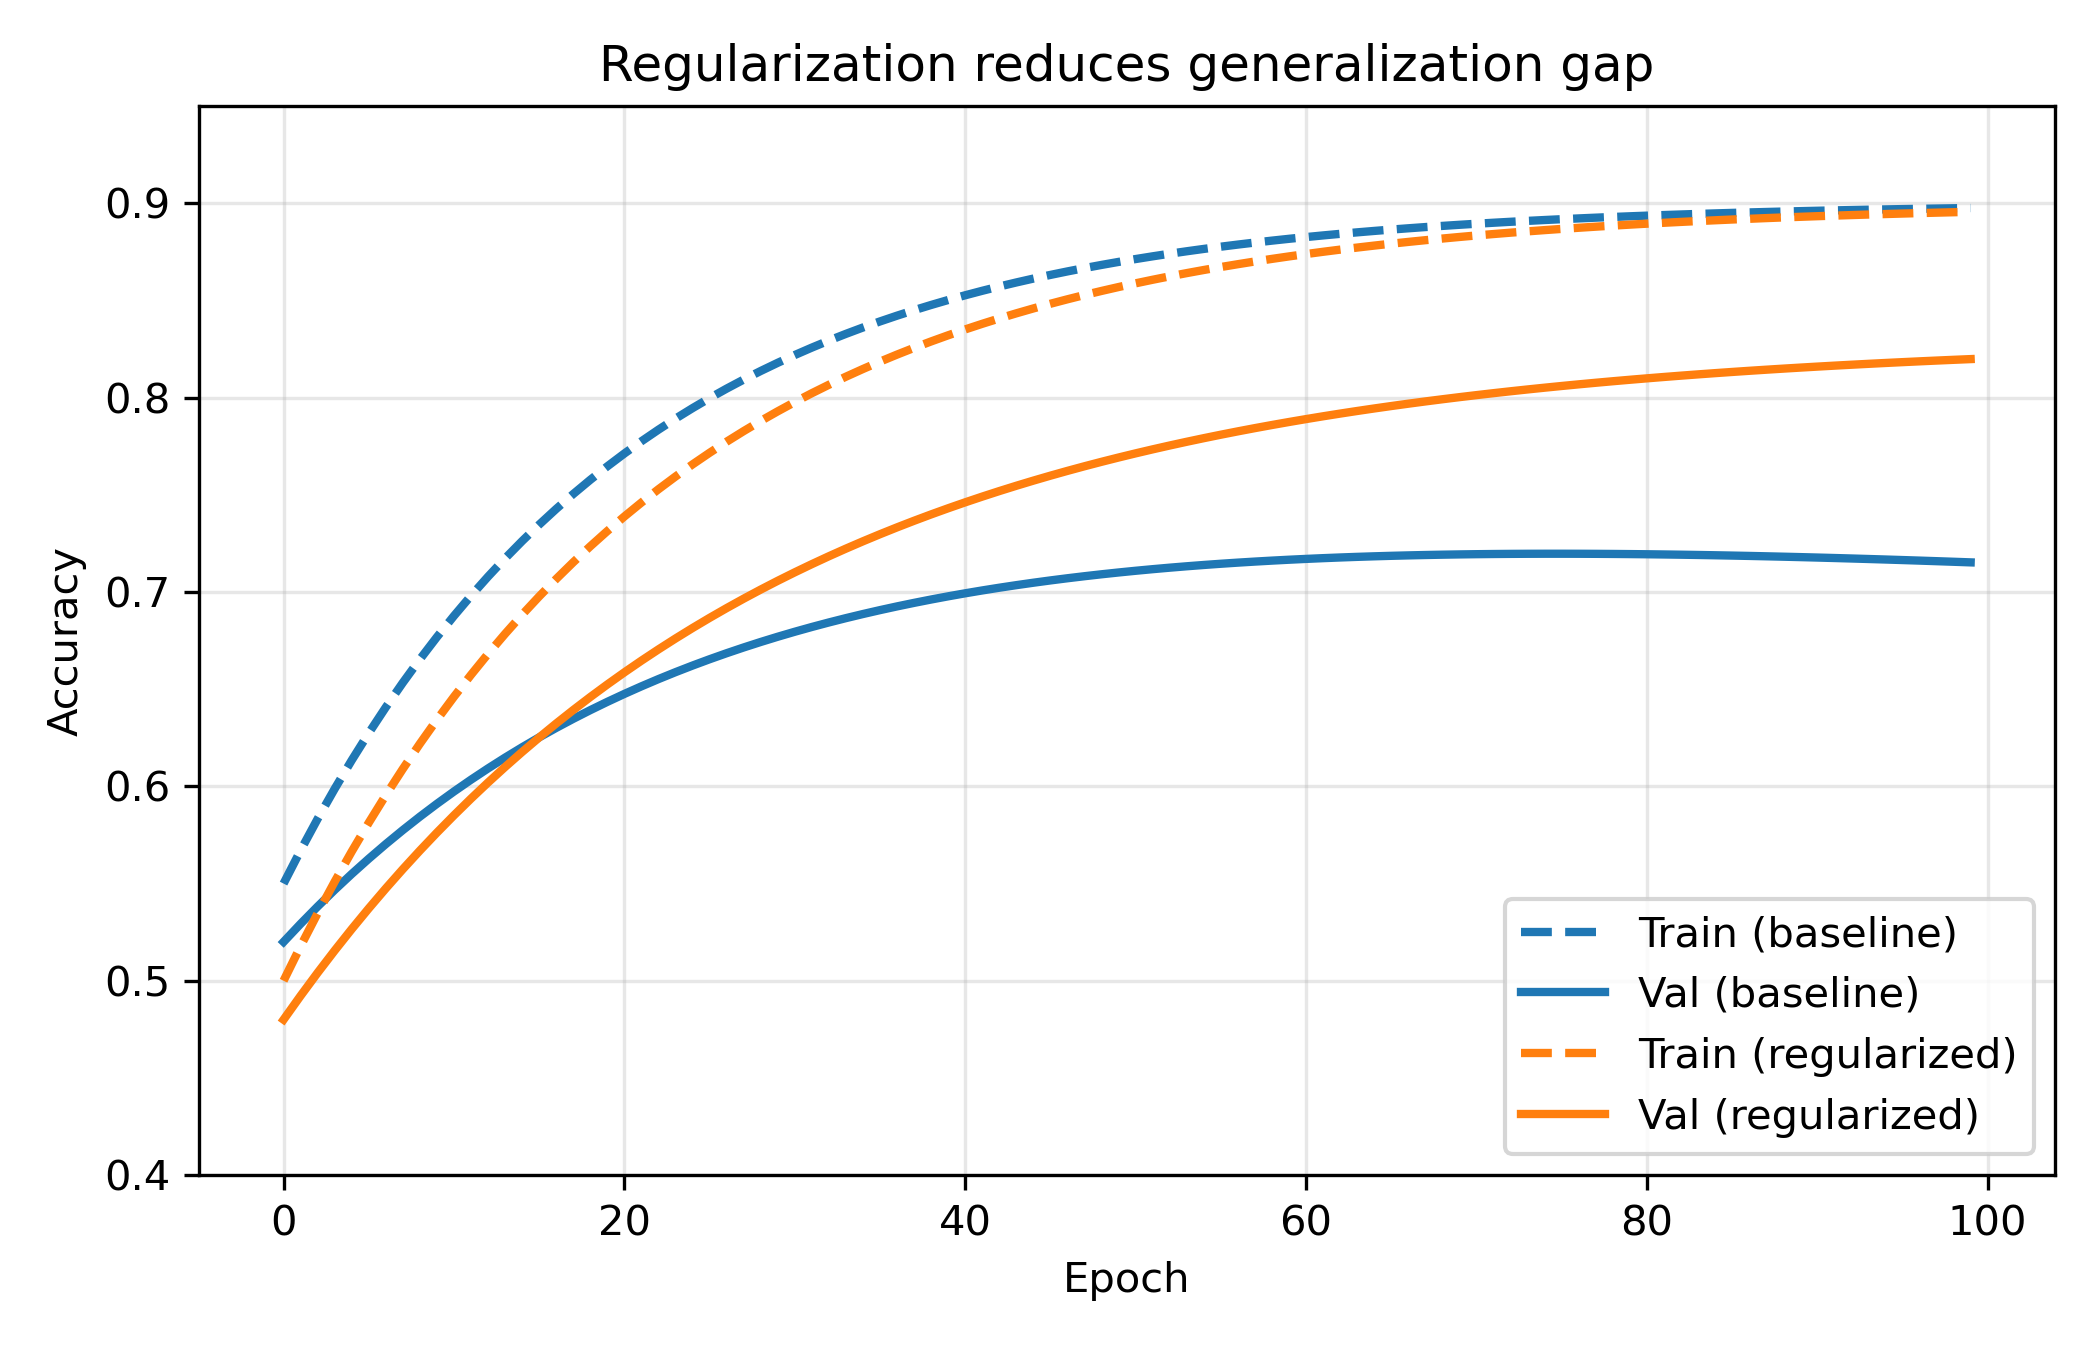
\includegraphics[width=0.8\linewidth]{regularization_effects.png}
  \caption{Validation accuracy trajectories illustrating regularization benefits.}
  \label{fig:regularization_effects}
\end{figure}
\FloatBarrier

\end{document}
